\begin{figure}[tbp]
\centering
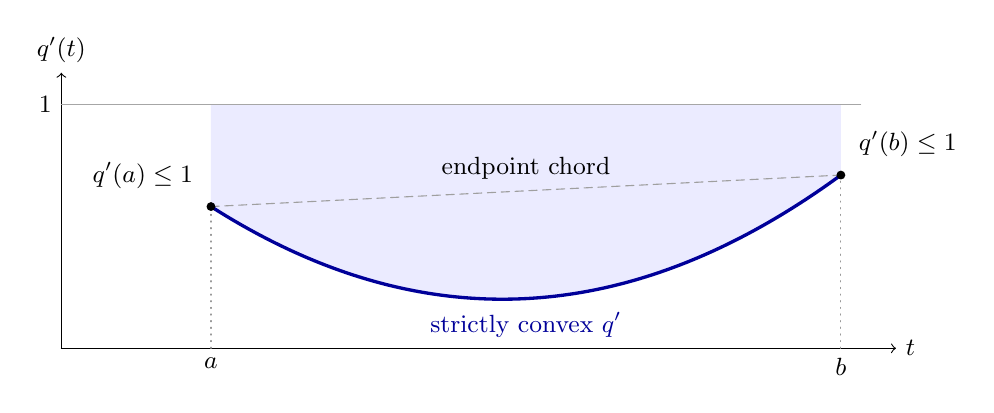
\begin{tikzpicture}[x=1cm,y=1cm,font=\small,line cap=round]
  \fill[blue!8] (0,3.1) -- (8,3.1) -- (8,2.2)
     .. controls (5.3333,.25) and (2.6667,.10) .. (0,1.8) -- cycle;
  \draw[->] (-1.9,0) -- (8.7,0) node[right] {$t$};
  \draw[->] (-1.9,0) -- (-1.9,3.5) node[above] {$q'(t)$};
  \draw[gray!70] (-1.9,3.1) -- (8.25,3.1);
  \node[left] at (-1.9,3.1) {$1$};
  \draw[densely dashed,gray!75] (0,1.8) -- (8,2.2)
    node[midway,above=3pt,text=black,fill=blue!8,inner sep=1pt]
       {endpoint chord};
  \draw[very thick,blue!60!black] (0,1.8)
    .. controls (2.6667,.10) and (5.3333,.25) .. (8,2.2);
  \draw[dotted,gray!80] (0,0) -- (0,1.8);
  \draw[dotted,gray!80] (8,0) -- (8,2.2);
  \fill (0,1.8) circle (1.6pt);
  \fill (8,2.2) circle (1.6pt);
  \node[below] at (0,0) {$a$};
  \node[below] at (8,0) {$b$};
  \node[above left=3pt] at (0,1.8) {$q'(a)\le1$};
  \node[above right=3pt] at (8,2.2) {$q'(b)\le1$};
  \node[below,blue!60!black] at (4,.58) {strictly convex $q'$};
\end{tikzpicture}
\caption{The contradiction on a hypothetical support gap with
$\gamma=c>0$. Strict convexity puts $q'$ below its endpoint chord,
which is at most $1$. The shaded deficit is positive, whereas contact
at both endpoints requires $\int_a^bq'(t)\,\dd t=q(b)-q(a)=b-a$.
The endpoint derivatives need not equal $1$.}
\label{fig:gap-convexity}
\end{figure}
